%! TEX root = guide.tex

% Possible arguments for the HKNdocument class:
% Language:
%   italian (default): Sets the document language to Italian.
%   english: Sets the document language to English.
%
% Table of Contents (ToC) depth:
%   toc=chapters: Shows only chapters in the ToC (tocdepth=0).
%   toc=sections: Shows chapters and sections in the ToC (tocdepth=1).
%   toc=subsections: Shows up to subsections in the ToC (default, tocdepth=2).
%   toc=subsubsections: Shows up to sub-subsections in the ToC (tocdepth=3).
%
% Font size:
%   10pt: Sets the base font size to 10 points.
%   11pt (default): Sets the base font size to 11 points.
%   12pt: Sets the base font size to 12 points.
%
% Draft mode:
%   draft: Compiles the document in draft mode (useful for proofreading, dummy images and imported files).
\documentclass[english,12pt,toc=sections]{HKNdocument}
% Packages
\usepackage{listings}                    % Code highlighting
\usepackage{xcolor}                      % Custom colors
\usepackage{longtable}                   % Breakable tables
\usepackage{ulem}                        % Underline
\usepackage{contour}                     % Border around text
\usepackage{tcolorbox}                   % Custom boxes

% Primary (Accent) Colors
% Primary (Accent) Colors
\definecolor{accentYellow}{RGB}{254, 196, 41}  % #FEC421
\definecolor{accentRed}{RGB}{236, 45, 36}      % #EC2D24

% Secondary Colors
\definecolor{supportOrange}{RGB}{242, 183, 5}  % #F2B705
\definecolor{supportDarkBlue}{RGB}{55, 81, 113} % #375171

% Background Colors
\definecolor{backgroundLight}{RGB}{242, 242, 242} % #F2F2F2

% Text & Border Colors
\definecolor{textGrayBlue}{RGB}{100, 117, 140}   % #64758C
\definecolor{textGrayMedium}{RGB}{146, 154, 166}  % #929AA6
\definecolor{textGrayLight}{RGB}{184, 187, 191}   % #B8BBBF



% Listings style
\lstdefinestyle{hkn}{
  basicstyle=\ttfamily\small\color{textGrayBlue},                         % Base style (size and font)
  keywordstyle=\bfseries\color{accentRed},           % Keywords in red (important, eye-catching)
  identifierstyle=\color{supportDarkBlue},               % Identifiers in blue (clear distinction)
  commentstyle=\color{textGrayMedium},                 % Comments in gray-blue (less prominent)
  stringstyle=\color{supportOrange},                 % Strings in orange (warm and readable)
  numberstyle=\ttfamily\scriptsize\color{textGrayMedium}, % Line numbers in gray (non-intrusive)
  backgroundcolor=\color{backgroundLight},           % Light background for contrast
  rulecolor=\color{textGrayLight},                   % Soft gray border for structure
  frame=single,                          % Border around code (single, double, shadowbox, none)
  framerule=0.8pt,                       % Border thickness
  frameround=tttt,                       % Round all corners
  framesep=5pt,                          % Distance between border and code
  rulesep=2pt,                           % Distance between border and code line
  numbers=left,                          % Line number position (left, right, none)
  stepnumber=1,                          % Line number interval
  numbersep=10pt,                        % Distance between line numbers and code
  xleftmargin=30pt,                      % Left margin
  xrightmargin=30pt,                     % Right margin
  resetmargins=true,                     % Reset margins
  numberblanklines=false,                % Number blank lines
  firstnumber=auto,                      % Initial line number
  columns=fixed,                         % Fixed column width
  showstringspaces=false,                % Show spaces in strings
  tabsize=2,                             % Tab size
  breaklines=true,                       % Automatic line break for long lines
  breakatwhitespace=true,                % Line break at whitespace
  breakautoindent=true,                  % Automatic indentation after line break
  escapeinside={(*@}{@*)}                % LaTeX commands in code
}

% Underline settings
\renewcommand{\ULdepth}{1.8pt} % Underline depth
\contourlength{0.8pt}

% Custom underline command
\newcommand{\myuline}[1]{%
\uline{\phantom{#1}}%
\llap{\contour{white}{#1}}%
}

% tcolorbox color settings
\definecolor{tcolorboxLeftColor}{RGB}{2, 65, 191}
\definecolor{tcolorboxBackTitleColor}{RGB}{119, 152, 255}
\definecolor{tcolorboxBackColor}{RGB}{210, 226, 255}

% Custom boxes
\newtcolorbox[auto counter, number within=chapter]{definition}[1]{
  title={\iflanguage{italian}{Definizione}{Definition}\par~\arabic{\tcbcounter}.~#1},
  boxrule=0mm,                       % Bordo principale (disabilitato)
  leftrule=1mm,                    % Bordo sinistro principale
  arc=2mm,
  colframe=accentRed,       % Colore bordo
  colbacktitle=textGrayMedium,
  colback=backgroundLight,        % Colore sfondo
  fonttitle=\bfseries,
  rounded corners=all,               % Bordi arrotondati
  }

\newtcolorbox[auto counter, number within=chapter]{theorem}[1]{
  title={\iflanguage{italian}{Teorema}{Theorem}~\arabic{\tcbcounter}.~#1},
  boxrule=0mm,                       % Bordo principale (disabilitato)
  leftrule=1mm,                    % Bordo sinistro principale
  arc=2mm,
  colframe=accentYellow,       % Colore bordo
  colbacktitle=textGrayMedium,
  colback=backgroundLight,        % Colore sfondo
  fonttitle=\bfseries,
  rounded corners=all,               % Bordi arrotondati
}

\newtcolorbox[auto counter, number within=chapter]{corollary}[1]{
  title={\iflanguage{italian}{Corollario}{Corollary}~\arabic{\tcbcounter}.~#1},
  boxrule=0mm,                       % Bordo principale (disabilitato)
  leftrule=1mm,                    % Bordo sinistro principale
  arc=2mm,
  colframe=supportOrange,       % Colore bordo
  colbacktitle=textGrayMedium,
  colback=backgroundLight,        % Colore sfondo
  fonttitle=\bfseries,
  rounded corners=all,               % Bordi arrotondati
}

\newtcolorbox[auto counter, number within=chapter]{exercise}[1]{
  title={\iflanguage{italian}{Esercizio}{Exercise}~\arabic{\tcbcounter}.~#1},
  boxrule=0mm,                       % Bordo principale (disabilitato)
  leftrule=1mm,                    % Bordo sinistro principale
  arc=2mm,
  colframe=supportDarkBlue,       % Colore bordo
  colbacktitle=textGrayMedium,
  colback=backgroundLight,        % Colore sfondo
  fonttitle=\bfseries,
  rounded corners=all,               % Bordi arrotondati
}

\newtcolorbox[auto counter, number within=chapter]{observation}[1]{
  title={\iflanguage{italian}{Osservazione}{Observation}~\arabic{\tcbcounter}.~#1},
  boxrule=0mm,                       % Bordo principale (disabilitato)
  leftrule=1mm,                    % Bordo sinistro principale
  arc=2mm,
  colframe=textGrayBlue,       % Colore bordo
  colbacktitle=textGrayMedium,
  colback=backgroundLight,        % Colore sfondo
  fonttitle=\bfseries,
  rounded corners=all,               % Bordi arrotondati
  }



\begin{document}
% Document metadata
\title{Guide to conventions and packages for the HKNotes project}
\shorttitle{HKNotes Guide}
% You can include multiple \autor commands to list all autors in the frontpage.
\author{Erik Scolaro}

% You can include multiple \editor commands to list all editors in the frontpage.

\docdate{\today}
\docversion{1.1}

\frontmatter
\maketitle
\cclicense
\tableofcontents
\clearpage

\mainmatter
\chapter{Introduction}

In this file, which has the same structure as the notes you will have to write, I will show you the basic usage of some packages and explain the structure of the project.

\section{Project Structure}

The project contains several folders:
\begin{itemize}
	\item \texttt{chapters}, where you will insert a .tex file for each chapter with the same name (you can also name them chapter 1, 2, but trust me, if you name them sensibly, it will be much easier to reorder them later);
	\item \texttt{res}, this folder will contain any source files of type \texttt{.gbb} from Geogebra and \texttt{.py} if you want to use Python for creating graphs. Every time you create a graph, you must save the source file in the corresponding folder. Additional folders will be added based on the future tools chosen for generating graphs or other resources.
	\begin{itemize}
		\item \texttt{gbb}, contains the Geogebra source file. It must be saved to ensure you can modify the corresponding graph in the future.
		\item \texttt{py}, I’ve prepared some .py scripts to evaluate the potential of using matplotlib for creating your graphs. Inside, you will also find a file named \texttt{run\_all\_scripts.py}, which allows you to run all other .py files in the folder and automatically generate all the graphs. Note that this solution avoids the issue of saving the graphs; in fact, the various examples you can take as base templates for your graphs automatically save in the \texttt{./res/svg} folder, with the same name as the .py file and in svg format.
		\item \texttt{svg}: this is where all the resources used within your notes will be placed, such as any svg files generated from Geogebra or Python or draw.io. draw.io is a powerful tool that allows you to intuitively and graphically create diagrams and electrical circuits. In this specific case, you don’t need to save both the source and the svg, just the file in .drawio.svg format, because it can be used both in LaTeX as svg and in draw.io for future modifications.
	\end{itemize}
	\item \texttt{template.tex}, this is where the magic happens. Basically, you only need to focus on organizing the chapters in the order you prefer, and you may need to modify a few small things that will be indicated to you as the project takes shape, such as inserting your information if you want to be credited and a brief explanation of the changes made to the document.
	\item Other files you don’t need to worry about are generated automatically by the compiler. The only significant one will be \texttt{main.pdf} or whatever you named the main file, which will be the compiled .pdf file and and it is located in the build folder in a folder named the same as the one that contains the project you are compiling.
\end{itemize}

\chapter{Graphs}
Here, I will simply show you how to import graphs in .svg format, add captions to them, and resize them properly.

\begin{figure}[!ht]
  \centering
  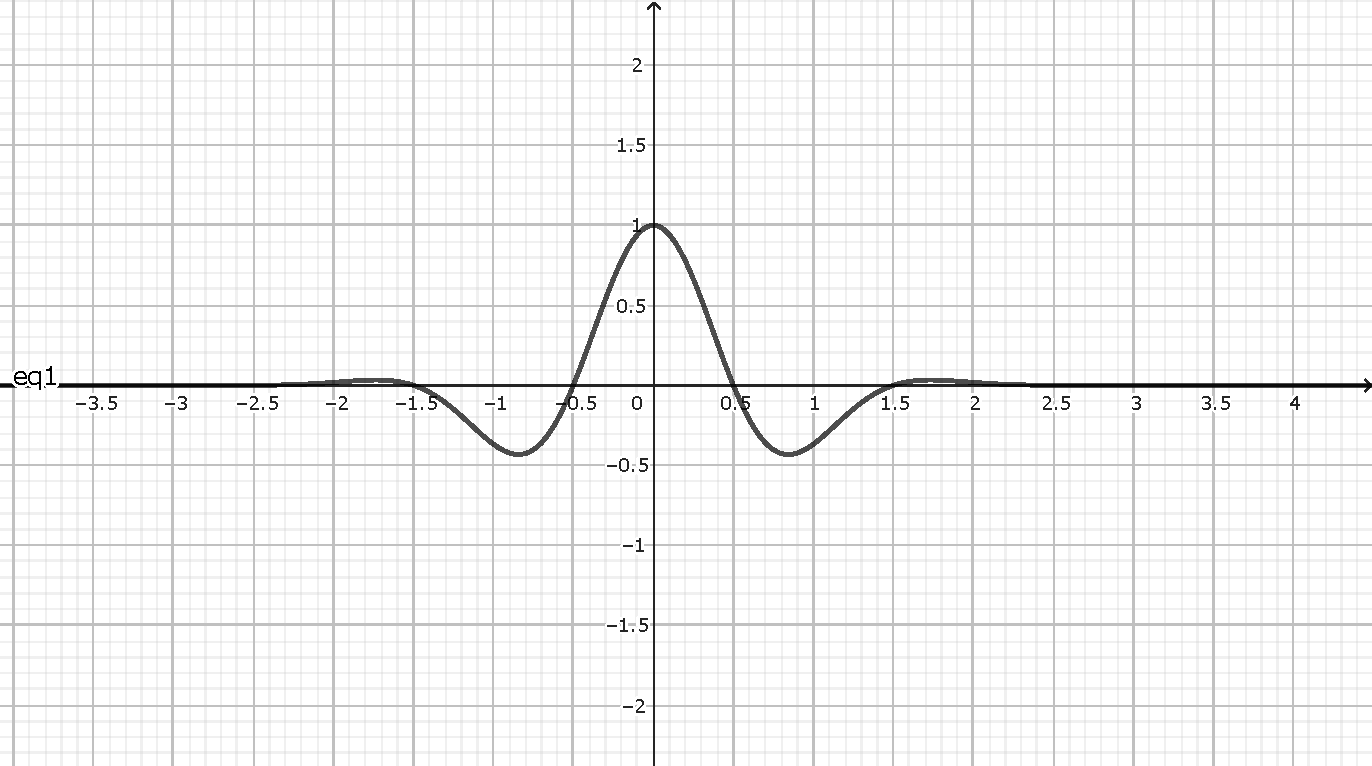
\includegraphics[width=0.8\textwidth]{svg-inkscape/esempio_geogebra_svg-raw.pdf}
  \caption{Example of including a PDF document.}
  \label{fig:pdf-example}
\end{figure}


\begin{figure}[!ht]
	\centering
	% Import the SVG image, applying cropping and resizing
	\includesvg[width=0.8\textwidth,inkscapelatex=false]{res/svg/esempio_geogebra}
	\caption{This is the example graph I created with Geogebra, with a caption and an associated label. To import SVG graphs, you need to install Inkscape, add it to the system path (watch out for the path, nothing works if you don’t do this, it’s usually \texttt{C:/Program Files/Inkscape/bin}), and modify the compiler flag by adding \texttt{-shell-escape}. If you are on Overleaf, it does this automatically (lucky you who didn’t waste 1 hour figuring this out, as a revenge, I write the most important things in the captions xD).}
	\label{graph:esempiografico}
\end{figure}

\hfill

\begin{figure}[!ht]
	\centering
	% Import the SVG image, applying cropping and resizing
	\includesvg[width=0.8\textwidth,inkscapelatex=false]{res/svg/2d_example}
	\caption{This is the 2d graph I created with matplotlib, see script.}
	\label{graph:esempiograficopy}
\end{figure}

\hfill

\begin{figure}[!ht]
	\centering
	% Import the SVG image, applying cropping and resizing
	\includesvg[width=0.8\textwidth,inkscapelatex=false]{res/svg/3d_continuous_example}
	\caption{This is the continuous 3d graph I created with matplotlib, see script.}
	\label{graph:esempiograficopy2}
\end{figure}

\hfill

\begin{figure}[!ht]
	\centering
	% Import the SVG image, applying cropping and resizing
	\includesvg[width=0.8\linewidth,inkscapelatex=false]{res/svg/3d_wireframe_example}
	\caption{This is the continuous 3d graph I created with matplotlib, see script.}
	\label{graph:esempiograficopy3}
\end{figure}

\hfill

\begin{figure}[!ht]
	\centering
	% Import the SVG image, applying cropping and resizing
	\includesvg[width=0.8\linewidth,inkscapelatex=false]{res/svg/esempioMappaConcettuale.drawio}
	\caption{A dummy conceptual map created with the draw.io online editor.}
	\label{graph:esempioMappaConcettuale}
\end{figure}

\hfill

\begin{figure}[!ht]
	\centering
	% Import the SVG image, applying cropping and resizing
	\includesvg[width=0.8\linewidth,inkscapelatex=false]{res/svg/esempioCircuito.drawio}
	\caption{A basic circuit created with the draw.io online editor.}
	\label{graph:esempioCircuito}
\end{figure}

\hfill

If you open the .tex file, you will notice that I have inserted the \texttt{\textbackslash href} command between each graph. This is to prevent \LaTeX from optimizing the space by fragmenting the bulleted list below between the graphs. Don’t believe me? Try it and see what chaos it creates.

Labels can be associated with many objects in Matlab, make good use of them! Especially when you need to refer to formulas, tables, or graphs in your text. Here are all the ways you can reference an object with an associated label:
\begin{enumerate}
	\item \texttt{\textbackslash ref\{graph:esempiografico\}}: To refer to the number associated with the label, such as a figure, table, section, etc. (example: Figure~\ref{graph:esempiografico}).
	\item \texttt{\textbackslash pageref\{graph:esempiografico\}}: To refer to the page number where the labeled object appears (example: See page~\pageref{graph:esempiografico}).
	\item \texttt{\textbackslash hyperref\{graph:esempiografico\}}: If you use the \texttt{hyperref} package, you can click the reference to go directly to the figure, table, etc.
	\item \texttt{\textbackslash eqref\{graph:esempiografico\}}: To refer to an equation, if the label has been applied to an equation environment (example: as shown in equation~\eqref{graph:esempiografico}).
\end{enumerate}

\chapter[Advanced Mathematics]{Assigning Labels to Equations in LaTeX and Citing Them Later}

I don't want to talk to you about how to write mathematics, there are millions of guides on this topic. Instead, I want to talk about the ability to assign labels to equations in LaTeX so that they can be cited later.

\section{Introduction}

One of LaTeX's most powerful features is the ability to assign labels to equations and then easily cite them within the document. This is particularly useful in scientific and technical documents, where it's often necessary to refer to specific equations. In this chapter, we will see how to label equations and how to cite them automatically, ensuring that the equation number is updated correctly during the document compilation.

\section{Assigning a Label to an Equation}

To label an equation, you need to use the \verb|\label{}| command within the environment where the equation is written (e.g., \verb|equation|, \verb|align|, etc.). The argument of the \verb|\label{}| command is the name of the label, which must be unique in the document.

Here's an example of labeling an equation:
\begin{quote}
\begin{verbatim}
\begin{equation}
\label{eq:energy}
    E = m c^2
\end{equation}
\end{verbatim}
\end{quote}

\begin{equation}
\label{eq:energy}
    E = m c^2
\end{equation}

In this case, the equation is labeled with \texttt{eq:energy}. Now, LaTeX will automatically assign a number to this equation, which can be cited later in the document.

\section{Citing an Equation}

To reference the labeled equation, use the \verb|\ref{}| command. The argument of the \verb|\ref{}| command is the name of the label that was assigned to the equation.

Here's how to cite the previous equation:

\begin{quote}
\begin{verbatim}
As shown in equation \ref{eq:energy},
Einstein's famous formula relates energy to mass.
\end{verbatim}
\end{quote}

The result will be:

\begin{quote}
    As shown in equation \ref{eq:energy},
    Einstein's famous formula relates energy to mass.
\end{quote}

LaTeX will automatically replace \verb|\ref{eq:energy}| with the equation number (e.g., \((1)\)), which will update if other equations are added or removed from the document.

\section{Citing an Equation with a Prefix}

If you want to add a prefix to the equation number (like ``Eq.'' or ``Equation''), you can do so manually. For example:

\begin{quote}
\begin{verbatim}
As shown in Eq.~\ref{eq:energy},
Einstein's famous formula relates energy to mass.
\end{verbatim}
\end{quote}

The result will be:

\begin{quote}
    As shown in Eq.~\ref{eq:energy},
    Einstein's famous formula relates energy to mass.
\end{quote}

\section{Citations with the \texorpdfstring{\texttt{align}}{align} Environment}

When using environments like \verb|align|, which allow you to write multiple equations on separate lines, you can label each individual equation. Here's an example:
\begin{align}
\label{eq:sum}
    a + b & = c \\
\label{eq:diff}
    x - y & = z
\end{align}

To cite the individual equations:

\begin{quote}
\begin{verbatim}
As shown in \ref{eq:sum} and \ref{eq:diff}, the operations of
addition and subtraction are defined respectively.
\end{verbatim}
\end{quote}

The result will be:

\begin{quote}
    As shown in \ref{eq:sum} and \ref{eq:diff},
    the operations of addition and subtraction
    are defined respectively.
\end{quote}

\section{Citing an Equation with the \texorpdfstring{\texttt{\textbackslash eqref}}{eqref} Command}

If you want to cite an equation including the parentheses around the equation number automatically, you can use the \verb|\eqref{}| command instead of \verb|\ref{}|. Here's how:

\begin{quote}
\begin{verbatim}
As shown in \eqref{eq:energy},
Einstein's formula expresses energy in terms of mass.
\end{verbatim}
\end{quote}

The result will be:

\begin{quote}
    As shown in \eqref{eq:energy},
    Einstein's formula expresses energy in terms of mass.
\end{quote}

\chapter{Formatting Code}

In this chapter, we will show how to use the \texttt{listings} package to format source code in LaTeX. This package allows you to highlight the syntax of various programming languages and customize the style to fit your document.

\section{Inserting Code}

After defining the style, you can use it to format code within the document. To do this, use the \texttt{\textbackslash lstset} command to set the style and the \texttt{\textbackslash lstinputlisting} or \texttt{\textbackslash begin{lstlisting}...\textbackslash end{lstlisting}} command to include the code. Here is an example:

\subsection{Example with External File} You can also include an external file containing the code:

\lstinputlisting[language=Python, style=hkn]{res/py/2d_example.py}

\section{Formatting the Code}

The \texttt{listings} package allows you to display source code within a LaTeX document while preserving formatting and syntax highlighting. In this section, we will explore how to use \texttt{listings} to include and format code in our document.

\subsection{Predefined Styles}

\texttt{listings} provides some predefined styles for syntax highlighting of various programming languages. These styles allow you to easily include code blocks with correct syntax highlighting.

For example, to include Python code in the document, you can use the following command:

\begin{lstlisting}
	\begin{lstlisting}[language=Python]
		def hello_world():
		print("Hello, World!")
  \end {lstlisting}
\end{lstlisting}

sdfgadfgfg
Result:
\begin{lstlisting}[language=Python]
	def hello_world():
	print("Hello, World!")
\end{lstlisting}

In this example, the \texttt{listings} package automatically recognizes Python syntax and highlights it correctly.

\subsection{Supported Programming Languages}

\texttt{listings} supports many programming languages, so you can use automatic syntax highlighting for a wide range of languages. Just specify the language using the \texttt{language} option within the \texttt{lstlisting} environment. Some supported languages include:

\begin{itemize}
	\item Python: \texttt{language=Python}
	\item C/C++: \texttt{language=C}
	\item Java: \texttt{language=Java}
	\item SQL: \texttt{language=SQL}
	\item HTML: \texttt{language=HTML}
	\item CSS: \texttt{language=CSS}
	\item JavaScript: \texttt{language=JavaScript}
	\item XML: \texttt{language=XML}
\end{itemize}

Example of SQL code:

\begin{lstlisting}[language=SQL]
	SELECT * FROM users WHERE age > 18;
\end{lstlisting}

\subsection{Customizing Styles}

Although the package offers predefined styles, it is possible to customize the appearance of the code. If there is a need to create new styles, contact the responsible person. Some customizable parameters, listed here to highlight the potential of the styles, include:

\begin{itemize}
	\item \texttt{language}: Defines the language of the code.
	\item \texttt{basicstyle}: Sets the base font for the code.
	\item \texttt{keywordstyle}: Modifies the style of keywords.
	\item \texttt{stringstyle}: Modifies the style of strings.
	\item \texttt{commentstyle}: Defines the style for comments.
	\item \texttt{numbers}: Displays line numbers.
	\item \texttt{frame}: Adds a border around the code.
	\item \texttt{backgroundcolor}: Sets the background color of the code.
\end{itemize}

This is the before and after applying the SQL style defined in HKNtools.tex:

\begin{lstlisting}[language=SQL]
	-- Query to select user data
	SELECT name, age
	FROM users
	WHERE age > 18
	ORDER BY age DESC;
\end{lstlisting}

\begin{lstlisting}[language=SQL, style=hkn]
	-- Query to select user data
	SELECT name, age
	FROM users
	WHERE age > 18
	ORDER BY age DESC;
\end{lstlisting}

\subsection{Global Configuration}

You can also configure \texttt{listings} globally to apply the same style settings throughout the document using the \texttt{\\lstset} command. For example:

\begin{lstlisting}
\lstset{
	language=Python,
	numbers=left,
	frame=single,
	backgroundcolor=\color{lightgray},
	stepnumber=1
}
\end{lstlisting}

This will set the options for all Python code blocks in the document.
Here are the effects before and after using the instruction:

\begin{lstlisting}[language=Python]
	def hello_world():
	print("Hello, World!")
\end{lstlisting}

\lstset{
	language=Python,
	numbers=left,
	frame=single,
	backgroundcolor=\color{lightgray},
	stepnumber=1
}

\begin{lstlisting}[language=Python]
	def hello_world():
	print("Hello, World!")
\end{lstlisting}

\section{Currently Defined Custom Styles}

Additional styles will be implemented as needed by collaborators. For now, the following styles are currently defined:

\begin{itemize}
	\item SQL: sqlstyle
\end{itemize}

\section{Complete Example}

Below is an example of a C program highlighted with the \texttt{listings} package. This program prints a greeting on the screen. As you can see, I used a \texttt{label} to easily reference the code later.

\begin{lstlisting}[language=C, style=hkn, caption={Demo}, label=code:demo]
#include <stdio.h>

int x = 10;
uint32_t y = 10;

// Example program
int main() {
  printf("Hello, World!\n");
  return 0;
}
\end{lstlisting}

This example is labeled with \texttt{label=code:demo}, so we can refer to this code anywhere in the document using the command \texttt{\ref{code:demo}}. For example, we can reference the code \ref{code:demo} in the text.

\chapter{Boxes}
\section{Boxing examples}

The numbering of the various boxes (such as Definitions, Theorems, Exercises, etc.) is automatically reset at the beginning of each chapter. This means that every time a new chapter starts, the box counter resets to 1, both for the boxes in Italian and those in English. It is important to note that the numbering of the boxes is independent between the two languages: if the command is used in Italian, the box will be numbered according to the Italian numbering system, while using the command in English will generate a box with an independent English numbering. As a result, the numbering between the Italian and English boxes is not synchronized. It is recommended to pay attention and maintain consistency in language usage to avoid confusion and ensure the numbering remains correct within each chapter.

\begin{definizione}{Un esempio di definizione}
  Questo è un esempio di una casella colorata con il titolo "Definizione" in italiano.
\end{definizione}

\begin{definition}{An example of a definition}
  This is an example of a colored box with the title "Definition" in English.
\end{definition}

\begin{teorema}{Un esempio di teorema}
  Questo è un esempio di una casella colorata con il titolo "Teorema" in italiano.
\end{teorema}

\begin{theorem}{An example of a theorem}
  This is an example of a colored box with the title "Theorem" in English.
\end{theorem}

\begin{corollario}{Un esempio di corollario}
  Questo è un esempio di una casella colorata con il titolo "Corollario" in italiano.
\end{corollario}

\begin{corollary}{An example of a corollary}
  This is an example of a colored box with the title "Corollary" in English.
\end{corollary}

\begin{osservazione}{Un esempio di osservazione}
  Questo è un esempio di una casella colorata con il titolo "Osservazione" in italiano.
\end{osservazione}

\begin{observation}{An example of an observation}
  This is an example of a colored box with the title "Observation" in English.
\end{observation}

\begin{esercizio}{Un esempio di esercizio}
  Questo è un esempio di una casella colorata con il titolo "Esercizio" in italiano.
\end{esercizio}

\begin{exercise}{An example of an exercise}
  This is an example of a colored box with the title "Exercise" in English.
\end{exercise}

\chapter{Tables with longtables}

\section{Longtable Example}
\begin{longtable}{|l|c|c|p{6.2cm}|}
    \caption{Example of a Longtable with Caption and Label}
    \label{tab:longtable_example}\\
    \hline \textbf{Concetto} & \textbf{Tipo} & \textbf{Volume} & \textbf{Motivazione}\\\hline
    \endfirsthead

    \hline \textbf{Concetto} & \textbf{Tipo} & \textbf{Volume} & \textbf{Motivazione}\\\hline
    \endhead

    \hline \multicolumn{4}{|r|}{{Continua all pagina successiva}}\\\hline
    \endfoot

    \hline
    \endlastfoot
    Utente                   & E             & 30.000.000      & {Ipotizziamo una piattaforma in cui sono iscritte 30 milioni di utenti}
    \\\hline
    Host                     & E             & 150.000         & {Ipotizziamo che sulla piattaforma si iscriveranno circa 150 mila host}
    \\\hline
    Alloggio                 & E             & 169.000         & {Ipotizziamo che nella piattaforma verranno registrati circa 169 mila alloggi}                                                                    \\\hline
    Prenotazione             & E             & 36.000.000      & {Ipotizziamo che sulla piattaforma siano state effettuate circa 36 milioni di prenotazioni}                                                               \\\hline
    Soggiorno                & E             & 34.920.000      & {Ipotizziamo che sulla piattaforma ci siano stati circa 35 milioni di soggiorni}                                                                  \\\hline
    Recensione               & E             & 12.000.000      & {Ipotizziamo che sulla piattaforma vengano scritte circa 12 milioni di recensioni}                                                                 \\\hline
    Commento                 & E             & 16.000.000      & {Ipotizziamo che sulla piattaforma vengano scritti circa 16 milioni di commenti}                                                                   \\\hline
    Lista                    & E             & 45.000.000      & {Ipotizziamo che sulla piattaforma vengano create circa 45 milioni di liste di alloggi preferiti}                                                                  \\\hline
    Servizio                 & E             & 20              & {Ipotizziamo che sulla piattaforma vengano messi a disposizione circa 20 servizi differenti}                                                                 \\\hline
    Possedimento             & R             & 169.000         & {Ipotizziamo che nella piattaforma ogni host abbia almeno un alloggio, e che 1 host su 8 abbia 2-3 alloggi}                                                                    \\\hline
    Richiesta                & R             & 36.000.000      & {Ipotizziamo che nella piattaforma 4 utenti registrati su 5 abbiano fatto almeno una prenotazione, e 1 su 5 ne abbia fatto almeno 3}                                                    \\\hline
    Generazione              & R             & 34.920.000      & {Ipotizziamo che sul totale delle prenotazioni, circa il 2\% vengano cancellate. Tutte le altre diventano soggiorni effettivi}                                                        \\\hline
    Elaborazione             & R             & 12.000.000      & {Ipotizziamo che 1 utente su 3 che ha effettuato una prenotazione poi scriva una recensione}                                                                 \\\hline
    Contenuto                & R             & 16.000.000      & {Ipotizziamo che circa 1 recensione su 3 abbia un thread con almeno 3 commenti e 1 su 3 abbia un solo commento}                                                                   \\\hline
    Creazione                & R             & 45.000.000      & {Ipotizziamo che circa 6 utenti su 10 creino delle liste, con una media di 2-3 liste per ciascuno di questi utenti}                                                                     \\\hline
    Scritto                  & R             & 16.000.000      & {Ipotizziamo che circa 1 utente su 5 abbia scritto un commento, e di questi uno ne abbia scritto circa 2-3}                                                                        \\\hline
    Correlazione             & R             & 12.000.000      & {Ipotizziamo che circa 1 soggiorno su 6 riceva una recensione da parte dell'utente o dell'host, e che 1 su 6 la riceva da parte di entrambi}                                           \\\hline
    Riserva                  & R             & 36.000.000      & {Ipotizziamo che tutti gli alloggi vengano riservati circa 36 milioni di volte, una volta per ogni prenotazione}                                                               \\\hline
    Offerto                  & R             & 250.000         & {Ipotizziamo che ogni alloggio offra più di una decina di servizi}                                                                    \\\hline
    Valutazione              & R             & 2.000.000       & {Ipotizziamo che circa 1 recensione su 3 viene scritta verso un alloggio}                                                                   \\\hline
\end{longtable}

\section{Syntax exaplanation}
The syntax used in LaTeX for the table \ref{tab:longtable_example} with the \texttt{longtable} package is as follows:

\begin{itemize}
    \item \textbf{Table Declaration}:
    \begin{verbatim}
    \begin{longtable}{|l|c|c|p{6.2cm}|}
    \end{verbatim}
    Here, a table is declared with 4 columns. The first column is left-aligned (\texttt{l}), the second and third columns are centered (\texttt{c}), while the fourth column has a width of 6.2 cm and adjusts to the content (\texttt{p\{6.2cm\}}).

    \item \textbf{Table Header}:
    \begin{verbatim}
    \hline \textbf{Concept} & \textbf{Type} & \textbf{Volume}
    & \textbf{Reason} \\\hline
    \end{verbatim}
    These lines are used to define the header of the table and separate it from the subsequent rows with a horizontal line.

    \item \textbf{Commands for Different Table Sections}:
    \begin{itemize}
        \item \texttt{endfirsthead}: Defines the header to be used on the first page of the table.
        \item \texttt{endhead}: Defines the header to be used on the following pages of the table.
        \item \texttt{endfoot}: Defines the footer for each page of the table.
        \item \texttt{endlastfoot}: Defines the final footer of the table.
    \end{itemize}

    \item \textbf{Data Rows}:
    Each data row is separated by \texttt{\\} and ends with \texttt{hline} to add a horizontal line after each row. The data in each cell is separated by \texttt{\&}.

    Example:
    \begin{verbatim}
    User & E & 30.000.000 & {Let’s assume a platform with 30
    million users} \\\hline
    \end{verbatim}







    This structure allows the creation of tables that can span multiple pages and contains horizontal lines in both the headers and between the data, maintaining a clear and readable format.
\end{itemize}


\backmatter

% input{_postamble.tex}
\end{document}
